%%=============================================================================
%% Methodologie
%%=============================================================================

\chapter{Methodologie}
\label{ch:methodologie}

%% TODO: Hoe ben je te werk gegaan? Verdeel je onderzoek in grote fasen, en
%% licht in elke fase toe welke stappen je gevolgd hebt. Verantwoord waarom je
%% op deze manier te werk gegaan bent. Je moet kunnen aantonen dat je de best
%% mogelijke manier toegepast hebt om een antwoord te vinden op de
%% onderzoeksvraag.


\section{Keuze algoritmen}
\label{sec:keuze-algoritmen}
Om goede resultaten te behalen is het uiterst belangrijk dat de juiste algoritmen gebruikt worden. Zo zijn er bepaalde algoritmen die helemaal niet bruikbaar zouden kunnen zijn voor deze casus. Er zal hier verder uitgelegd worden hoe we een mogelijk algoritme kunnen vinden.

\subsection{Superviseerd vs Ongesuperviseerd leren}
\label{sec: superviseerd-vs-ongesuperviseerd-leren}
Machine learning kan onderverdeelt worden in verschillende types van algoritmen. Deze zijn gesuperviseerd leren, ongesuperviseed leren en reinforcement leren. Dit laatste type is niet van toepassing voor deze casus. Met dit type wordt er geleerd op basis van positieve signalen (beloningen). Er wordt ook niet gebaseerd op een dataset en aangezien wij in bezit zijn van datasets is dit type overbodig om verder te onderzoeken. 

\subsection*{Superviseerd leren}
\label{sec: superviseerd-leren}
Dit type heeft als doel om een hypothese te bekomen die dan zal kunnen gebruikt worden om nieuwe ongekende input toe te wijzen aan een label die voorkwam in de eerdere trainingsdataset. De trainingsdataset bestaat uit verschillende parameters en een label. Onder dit type kan je algoritmen vinden die voor zowat alle cases gebruikt kunnen worden. Deze zijn echter wel nog opgedeeld in drie verschillende categorieën. Zo kan je een nieuwe waarde voorspellen op basis van vroegere resultaten, dit wordt regressie genoemd. Verder heb je classificatiealgoritmen hiermee kan een input toegewezen worden aan een bepaalde klasse met een label. En als laatste bestaan er clusteringsalgoritmen hiermee kan je ook onderverdelingen maken in klassen maar deze hebben geen label. Clustering en classificatie lijken op elkaar maar met classificatie weten we ook precies wat de data voorstelt. 

\subsection*{Ongesuperviseerd leren}
\label{sec: ongesuperviseerd-leren}
Verschillend met gesuperviseerd leren beschikt een ongesuperviseerd algoritme over een ongelabelde dataset. Er zijn verschillende inputs/parameters maar die behoren niet tot een specifieke klasse. Met dit type is het dan ook enkel maar mogelijk om aan clustering te doen. Als we dit willen toepassen voor deze casus is dit geen optimale manier. We kunnen wel bepaalde besturingsevents clusteren waardoor je tot een x aantal clusters kan komen maar we hebben geen idee of de ene cluster PacMan of Mortal Kombat is bijvoorbeeld. 


\textbf{\underline{{\Large misschien een voorbeeldje uitwerken? }}}


\section{Gesuperviseerde classificatie algoritmen}
\label{sec:gesuperviseerde-classificatie-algoritmen}

In deze casus beschikken we over een gelabelde dataset. Het doel is om met een gegeven input een concreet spel te krijgen als output. Doordat we een gelabelde dataset hebben en er verdelingen moeten gemaakt worden op basis van labels is een gesuperviseerd classificatiealgoritme de meest geschikte voor dit onderzoek. Op deze manier kunnen we ongekende input plaatsen bij één bepaald spel.


\subsection{Logistische regressie}
\label{sec:logistische-regressie}

Logistische regressie is het eerste algoritme die we zullen bespreken in deze bachelorproef. Ondanks de naam doet vermoeden, valt dit algoritme niet onder de categorie regressie zoals we in sectie \ref{sec: superviseerd-leren} superviseerd-leren hebben gezien. Dit is wel degelijk een classificatiealgoritme die echter wel gebruik maakt van de logistische functie. Aan de hand van die hypothese kunnen er voorspellingen gemaakt worden. Gedurende het trainingsproces wordt de hypothese geoptimaliseerd. Er zullen meerdere spelletjes voorzien zijn op de arcademachine dus ook meerdere klassen. Omdat we van nul af aan starten zal ook de binaire logistische regressie gebruikt worden en vervolgens zal een van de twee mogelijke methoden om met meerdere klassen te werken gebruikt worden. 

\subsubsection{Binaire logistische regressie}
\label{sec:Binaire-logistische-regressie}

Er moeten enkele puntjes uitgelegd worden voordat we aan de effectieve uitleg kunnen beginnen. Eerst en vooral moeten we weten wat we willen voorspellen. Aangezien we beginnen met binaire logistische regressie maken we een voorspelling tussen twee klassen. Onze vraag kan dus als volgt luiden "Speelt de gebruiker Mortal Kombat of niet?". De waarde \textit{y} zal ons het resultaat geven. \textit{Y} kan slechts twee waarden aannemen $y \; \in \; \{0,1\}$ met 1 als de positieve klasse, Mortal Kombat. Als \textit{y} 0 is dan duidt het op de negatieve klasse, in onze data stelt dit Pacman voor. 

Logistische regressie start vanuit de hypothese van lineaire regressie die als volgt is: 
$$
h(x_{i}) \:= \: \theta^{T}x_{i} \:=\: \theta_{0} \:+ \:\theta_{1}x_{i1} \:+ \: ...\: + \: \theta_{n}x_{in}
$$
$ \theta^{T}$ is de getransponeerde vector van parameters die door het algoritme gegenereerd worden. Als de uitkomst van deze vergelijking $\geq 0$ dan zal de positieve klasse voorspelt worden, de andere klasse zal dan gegeven worden wanneer $h(x) < 0$. 

De logistische regressie is niet meer dan de sigmoïd functie van die lineaire hypothese. Zo krijgen we $h(x) = g(\theta^{T}x)$ . De sigmoïd functie wordt ook wel logistische functie genoemd. Vandaar de naam logistische regressie. 
$$
g(x) \: = \: {\frac{1}{1+e^{-x}}} \: => \: h(x) \: = \:{\frac{1}{1+e^{-\theta^{T}x }}}
$$

De eigenschap van een sigmoïd functie is dat het resultaat altijd zal voldoen aan volgende voorwaarde: $ 0 \leq h(x) \leq1$. 
Nu weten we nog niet wat de waarde van $h(x)$ voor logistische regressie precies uitdrukt. Dit kunnen we wiskundig uitdrukken als $P(y=1|x;\theta)$. M.a.w. de kans dat $y = 1$ voor de gegeven vector \textit{x} met de parameters $\theta$. Wanneer je de kans op de negatieve klasse wenst te weten doet u eenvoudig weg $1 - P(y=1|x;\theta)$. 
\textit{X} kan nu gemakkelijk geclassificeerd worden. Wanneer $h(x)\,\geq\,0.5$ heeft \textit{x} de meeste kans om tot de positieve klasse te behoren in dit geval Mortal Kombat. Anderzijds als $h(x)\:<\:0.5$ zal \textit{x} behoren tot de negatieve klasse. 

\begin{figure}
	\centering
	\begin{tikzpicture} 
	\begin{axis}[
	axis lines = left,
	xlabel = {$\theta^{T}x_{i}$},
	ylabel = {$g(h(\theta^{T}(x))$},
	]
	%Below the red parabola is defined
	\addplot [
	samples=100, 
	color=red,
	]
	{1/(1+exp(-x)};
	%\addlegendentry{$-ln(x)$}
	\end{axis}
	\end{tikzpicture}
	\caption{Sigmoïd functie, wanneer  $\theta^{T}x_{i} = 0$ zal de sigmoïd functie gelijk zijn aan 0.5 dit wil zeggen dat de 2 klassen even veel kans hebben om gekozen te zijn. Naar mate  $\theta^{T}x_{i}$ van waarde verhoogt zal de waarschijnlijkheid voor de positieve klasse ook verhogen. }
	\label{fig:sigmoid-functie}
\end{figure}
 

\subsubsection{Multiklasse logistische regressie}
\label{sec:Multiklasse-logistische-regressie}
Wat u uit de naam al kan afleiden is dat dit een algoritme is om een classificatie te maken over meerdere klassen. Dit kan op twee methoden gedaan worden. De one-vs-one methode of de one-vs-rest(/all) methode. 
\subparagraph{One-vs-all}
Dit is de gemakkelijkste van de twee methoden. Zoals de naam al doet vermoeden vergelijken we één klasse tegenover alle andere klassen. Als er \textit{n} aantal klassen zijn dan zullen er \textit{n} hypothesen $h^{(\,k\,)}$ met $k \in \{\,Pacman, \, Mortal \:Kombat, \, Tetris, \,..\}$ gemaakt worden. \textit{k} is dan de positieve klasse en alle andere klassen samen is dan één negatieve klasse. \newline
Voor een nieuwe input \textit{x} die moet geclassificeerd worden gaat de methode als volgt te werk. $h^{(k)} (x)$ geeft een waarde terug die de waarschijnlijkheid uitdrukt dat x tot de klasse \textit{k} behoort. Dit wordt voor alle \textit{n} hypothesen gedaan. De klasse met de hoogste waarschijnlijkheid wordt dan logischerwijs gekozen als de voorspelde klasse waar \textit{x} toe behoort. 
\subparagraph{One-vs-one}
Met deze techniek vergelijken we twee klassen met elkaar zoals we gezien hebben in sectie \ref{sec:Binaire-logistische-regressie} binaire logistische regressie. Er worden dus opnieuw meerdere hypothesen gemaakt maar anders dan in one-vs-all worden er nu combinaties van twee klassen gebruikt wat er zo uitziet $h^{(\,k,\,m)}$. \textit{k} is in dit geval de positieve klasse en \textit{m} de negatieve. In totaal zullen er $n(n-1)/2$ hypothesen gemaakt worden.
om te bepalen tot welke klasse een nieuwe input \textit{x} behoort berekenen we $h^{(k,m)}(x)$ wanneer het resultaat $\geq 0.5$ krijgt de positieve klasse (\textit{k}) een "punt". Dit gebeurt voor alle hypothesen en de klasse met het meest aantal punten zal uiteindelijk het resultaat zijn van het algoritme. 

\subsubsection{Optimaliseren van algoritme}
\label{sec:Optimaliseren-algoritme}
Om een zo optimaal mogelijk algoritme te verkrijgen moet er gebruik gemaakt worden van optimalisatietechnieken. Gradiënt descent is zo'n techniek die de parameters $\theta$ optimaliseert om een zo'n correct mogelijke hypothese te krijgen. Voordat gradient descent besproken wordt gaan we eerst de kostfunctie bespreken. 

\paragraph{Kostfunctie logistische regressie}
\label{par:kostfunctie-log}
Een kostfunctie wordt genoteerd als $J(\theta)$. Die functie drukt de gemiddelde kost van de trainingsset met parameters $\theta$ uit. Aan de hand van gradient descent is het dan mogelijk om de parameters te optimaliseren zodat de kostfunctie geminimaliseerd wordt. Hoe lager de kostfunctie is hoe beter de hypothese.
De kostfunctie voor logistische regressie ziet er als volgt uit: 
$$ 
J(\theta) \; = \frac{1}{m}\sum_{i=1}^{m} \;   Kost (h_{\theta}(x^{(i)}), y^{(i)} )  
$$

De kost wordt als volgt berekent:
$$Kost (h_{\theta}(x), y) \; = \; -y\ln(h_{\theta}(x)) \;- \;(1-y) \ln(1-h_{\theta}(x))  \;\;\;\; met \; y \in \{0,1\}$$

We stellen \textit{y} gelijk aan 1. Dan zien we dat eigenlijk enkel het eerste deel van de functie ($-y\ln(h_{\theta}(x))$) van belang zal zijn want het tweede deel ($- (1-y) \ln(1-h_{\theta}(x))$ zal nul zijn omdat 1-\textit{y} dan nul zal zijn en dus het product ook nul is. Zo krijgen we: 
\newline $Kost (h_{\theta}(x), y) \; = \; -\ln(h_{\theta}(x))$. Op deze manier komen we uit bij de rode kostfunctie die u ziet in figuur \ref{fig:kostfunctie} p\pageref{fig:kostfunctie}.

$h_{\theta}(x)$ is de hypothese die uitgelegd is in \ref{sec:Binaire-logistische-regressie} binaire logistische regressie. Dus die drukt de waarschijnlijkheid uit dat een vector \textit{x} positief of negatief is. Wanneer we een perfect voorspelling willen dan zou de kost 0 moeten zijn enkel zo ben je volledig zeker dat het label die aan \textit{x} wordt toegekend 100\% positief of negatief is. Als de hypothese zo goed als zeker is dat het vector positief is zal de kost nog dicht bij nul zijn. Eens $h(x) > 0.5$ zal de kost sneller stijgen. Ditzelfde principe geldt voor de negatieve voorbeelden. 

De kostfunctie in één uitdrukking is: 
$$ 
min \;\; -\frac{1}{m}\;\sum_{i=1}^{m} \;  y^{(i)}\ln(h_{\theta}(x^{(i)})) \;- \;(1-y^{(i)}) \ln(1\:-\:h_{\theta}(x^{(i)}))  
$$

Er zijn nog andere kostfuncties die gebruikt kunnen worden maar deze wordt in het algemeen altijd gebruikt.
De functie kan afgeleid worden door een principe binnen statistiek namelijk het 'maximum likelihood estimation'-principe Dit is een manier om parameters te zoeken voor verschillende modellen zoals logistische regressie. Deze functie is ook convex. Convex is een eigenschap die gebruikt wordt voor optimalisatiefuncties. Dit houdt onder meer in dat de functie het globaal minimum bereikt. 

\begin{figure}
	\centering
		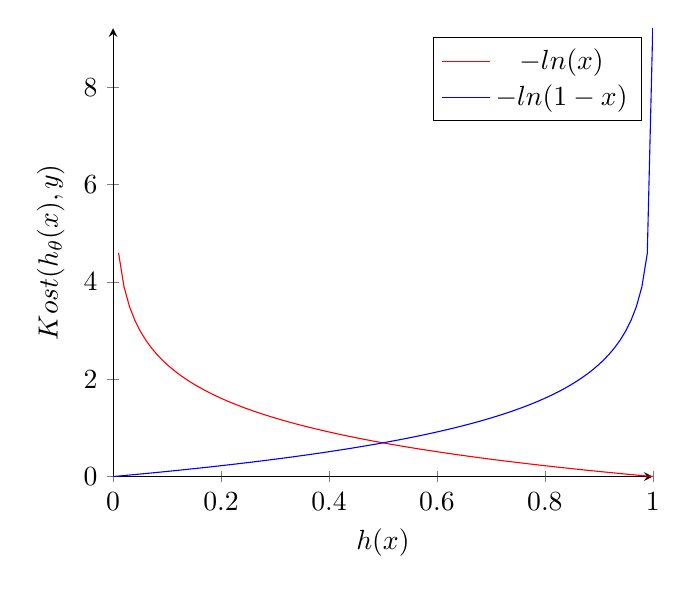
\begin{tikzpicture} 
		\begin{axis}[
		axis lines = left,
		xlabel = {$h(x)$},
		ylabel = {$Kost (h_{\theta}(x), y)$},
		]
		%Below the red parabola is defined
		\addplot [
		domain=0:1, 
		samples=100, 
		color=red,
		]
		{-ln(x)};
		\addlegendentry{$-ln(x)$}
		%Here the blue parabloa is defined
		\addplot [
		domain=0:1, 
		samples=100, 
		color=blue,
		]
		{-ln(1-x)};
		\addlegendentry{$-ln(1-x)$}
		
		\end{axis}
		\end{tikzpicture}
	\caption{Visualisatie functies}
	\label{fig:kostfunctie}
\end{figure}

\subsubsection{Gradient descent}
\label{sec:gradient-descent}
Gradient descent is een optimalisatiealgoritme die veel gebruikt wordt voor logistische regressie. Op deze manier is het mogelijk om de parameters $\theta$ te minimaliseren zodat de hypothese goede voorspellingen kan doen.
Gradient descent vereist een continue afleidbare functie, de kostfunctie die we zonet besproken hebben voldoet aan die vereisten. Er is ook een functie \textit{g} nodig die een vector teruggeeft als gradiënt en een stapgrootte $\alpha$. De stapgrootte zorgt ervoor dat het algoritme naar een lokaal of globaal minimum kan convergeren. Wanneer het algoritme stopt in een lokaal minimum heb je niet altijd de beste oplossing tenzij het lokaal minimum ook het globaal minimum is. Indien dit niet het geval is kan gradient descent een aantal keer herhaald worden zodat het globaal minimum kan gevonden worden. Het belang van een goede stapgrootte $\alpha$ is belangrijk. Wanneer die te groot is dan zou het kunnen dat het algoritme in een oneindige lus geraakt. Of als $\alpha$ te klein is dan kan het zeer lang duren tegen dat er een lokaal minimum gevonden is. 

Voor iedere parameter $\theta_{n}$ wordt volgende uitdrukking berekent en terug toegekend aan zichzelf. Tot de parameter amper nog verbetert. In implementaties is het mogelijk om te zeggen dat gradient descent moet stoppen wanneer het verschil van de nieuwe en oude parameter onder een bepaalde grens ligt. 
$$
\theta_{i} = \theta_{i} - \alpha\:\frac{\partial}{\partial\theta_{i}}(J(\theta_{i}, ... , \theta{n}))
$$

Deze functie kan afgeleid worden naar 
$$
\theta_{i} = \theta_{i} - \alpha\:\sum_{i=1}^{m}(h_{\theta}(x^{(i)})\:-\:y^{(i)} ) x_{j}^{(i) }
$$

\textbf{\textit{(Misschien nog voorbeeldje uitwerken en lokaal/globaal minimum uitleggen)}}


\subsection{Support Vector Machine}
\label{sec:Support-Vector-Machine}
Support Vector Machine is een volgend gesuperviseerd leeralgoritme die zal besproken worden. 
Andrew Ng is professor aan de Stanford University begon het deel support vectormachine in zijn cursus \autocite{cursusAndrewNg} met volgende zin.
\begin{quote}
	SVMs are among the best (and many believe are indeed the best) ‘off-the-shelf’ supervised learning algorithms.
\end{quote}

SVMs scoren over het algemeen beter dan logistische regressie of neurale netwerken. Het is uiteraard mogelijk dat een van die twee beter scoort maar dit is allemaal afhankelijk van de dataset. Vandaar dat het een logische keuze is om dit algoritme te vergelijken met ons vorige, logistische regressie. 

We maken gebruik van figuur \ref{fig:svm} op pagina \pageref{fig:svm} om de werking van een SVM uit te leggen. Daarna zal de kostfunctie uitgelegd worden die gebruikt wordt om het algoritme te optimaliseren. Dit alles is vereenvoudigd zodat het al mens makkelijker in te beelden is.
Het concept van SVM klinkt eenvoudig. De bedoeling is om een hyperplane te vinden die tussen de dichtstbijzijnde vector van een klasse en de hyperplane een zo groot mogelijke marge heeft. U ziet in de figuur dat het mogelijk is om meerdere hyperplanes te tekenen maar niet iedere hyperplane heeft een even grote marge. Om de marge beter te begrijpen gaan we eventjes terug naar logistische regressie. Daar kregen we een waarschijnlijkheid dat vector \textit{x} van een bepaalde klasse is. Als $\theta^{T}x \geq 0$ was $y=1$ en vice versa. Het is logisch dat hoe verder $\theta^{T}x$ van 0 ligt hoe zekerder de klasse kan toegekend worden. Dit is net wat SVM bijbrengt, een marge zodat je vanaf een bepaalde zekerheid, marge, pas een klasse toekent. Een marge wiskundige noteren is als volgt: $\theta^{T}x^{i} \ll 0$. $\ll$ betekent veel minder. Deze uitdrukking geldt dus voor $y^{i}=0$
 
Eerst en vooral wordt er een hyperplane gezocht die twee klassen van elkaar onderscheid. Zoals je in de figuur ziet is het mogelijk om meerdere hyperplanes (A,B) te maken. Die hyperplanes zijn van de vorm $h_{w,b}(x) = w^{T}x + b$ $w$ stelt nu $\theta_{n}^{T}$ voor en $b$ stelt $\theta_{0}$ voor. \textit{y} is nu geen element meer van {0,1} maar wel van {1,-1}. Als $h_{w,b}(x) > 1$ dan kunnen we stellen dat voor vector x een positieve klasse kan voorspelt worden. 
We nemen nu hyperplane \textit{A} om verder op te bouwen. We weten ook dat \textit{A1} het functie voorschrijft $w x +b=1$ heeft en \textit{A2} dan  $w x +b=-1$. Op deze manier is het mogelijk om de marge tussen \textit{A1} en \textit{A2} te berekenen. En die dus te optimaliseren.

\begin{figure}[]
	\centering
	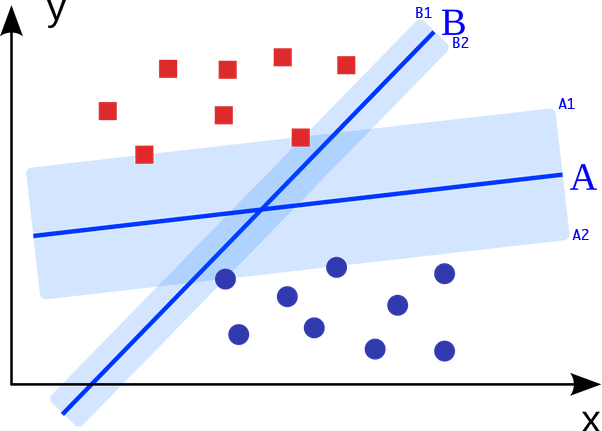
\includegraphics[width=0.6\textwidth]{img/svmkopie}
	\caption{Begeleidende afbeelding SVM \autocite{svmGraph}}
	\label{fig:svm}
\end{figure}

\subsubsection{Kostfunctie Support Vector Machine}

De kostfunctie van een SVM is gelijkaardig als de kostfunctie van logistische regressie. Er zijn enkele verschillen. Hier ziet u nog eens deze van logistische regressie: 
$$ 
min \;\; -\frac{1}{m}\sum_{i=1}^{m} \;  y^{(i)}\ln(h_{\theta}(x^{(i)})) \;- \;(1-y^{(i)}) \ln(1-h_{\theta}(x^{(i)}))  
$$
en de kostfunctie van een support vector machine is: 
$$ 
min \;\; C\sum_{i=1}^{m} \; \left[ y^{(i)}\;cost_{1}(\theta^{T}(x^{(i)})) \;- \;(1-y^{(i)})\;cost_{0}(\theta^{T}\:(x^{(i)})) \right] 
$$

Er zijn 2 grote wijzigingen. Het gedeelte $\ln(h_{\theta}\:(x^{(i)}))$ en $\ln(1-h_{\theta}\:(x^{(i)}))$ zijn vervangen door respectievelijk $cost_{1}\:(\theta^{T}\:(x^{(i)}))$ en $cost_{0}\:(\theta^{T}\:(x^{(i)})) $ 
Die kost functies kan u zien in figuren \ref{fig:cost1} en \ref{fig:cost0}. Als u de functies bekijkt zie u dat er eerst een plat stuk is en dan pas vanaf 1 of -1 begint te stijgen. Dit komt door de marge die we eerder besproken hebben. Wanneer  $\theta^{T}\:(x^{(i)}) \geq 1$ dan kunnen we ervan uit gaan dat $y=1$.
\begin{figure}
	\centering
	\begin{minipage}{.5\textwidth}
		\centering
		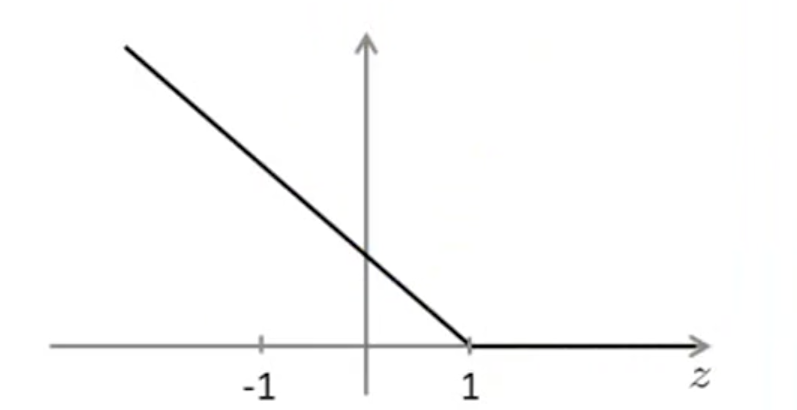
\includegraphics[width=1\linewidth]{img/costEen}
		\caption{$cost_{1}\:(\theta^{T}(x^{(i)}))$}
		\label{fig:cost1}
	\end{minipage}%
	\begin{minipage}{.5\textwidth}
		\centering
		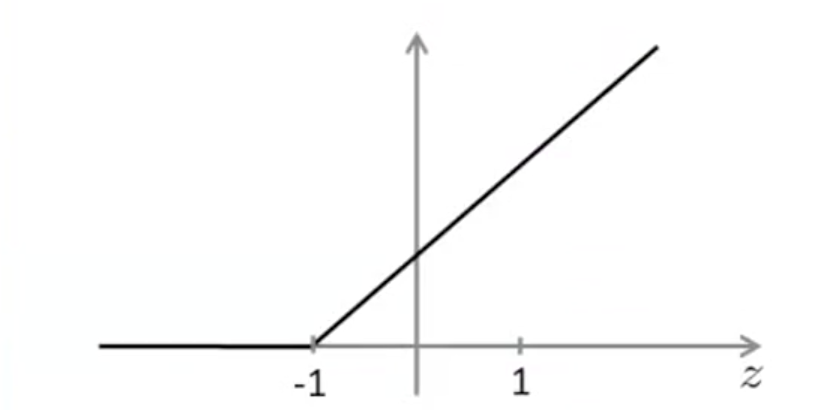
\includegraphics[width=1\linewidth]{img/costNul}
		\caption{$cost_{0}\:(\theta^{T}(x^{(i)})) $}
		\label{fig:cost0}
	\end{minipage}
\end{figure}


\subsection{Selectiecriteria}
\label{sec:Selectiecriteria}
Hoe weten we nu welk algoritme het best is om voorspellingen te doen op de arcade machine? We bespreken enkele selectiecriteria zodat de 2 algoritmen die we zonet besproken hebben kunnen vergelijken. 
Er zijn twee belangrijke factoren die beslissen of dat het ene algoritme beter is dan het andere voor een bepaalde dataset. 
Als we de algoritmen gaan implementeren dan zal altijd exact dezelfde dataset en testset gebruikt worden. De algoritmen worden beiden geïmplementeerd in Visual Studio 2015 en worden gerund zonder dat er een ander programma openstaat of draait in de achtergrond. Tussen de test wordt er ook nooit een ander programma geopend want het is altijd mogelijk dat die daarna nog in de achtergrond processen uitvoert. 

\subsubsection{Snelheid}
Snelheid is uiteraard een van de belangrijkste voorwaarden om een goed algoritme te zijn. Je wilt bijvoorbeeld geen 2 minuten wachten tegen dat je krijgt te weten wat de computer dacht dat je aan het spelen was. Een programma bestaat uit verschillende delen. Niet alle onderdelen van een programma zijn relevant voor deze bachelorproef. Zo heb je bijvoorbeeld het inlezen van de data. Dit proces zal even veel tijd in beslag nemen voor logistische regressie als voor vector support machine doordat dezelfde data gebruikt wordt voor beiden. Een tweede deel is natuurlijk de declaratie van variabelen en objecten dit gebeurt zodanig snel dat dit irrelevant is.\newline
Dan heb je het leerproces of optimalisatieproces van een algoritme. Dit is wel belangrijk want hiermee kan het verschil gemaakt worden. Daarvoor gebruiken we de klasse Stopwatch die in het .NET framework voorzien is. Die wordt gestart net voor de start van het leerproces en gestopt net erna. Op deze manier kunnen we precies meten hoelang het algoritme nodig heeft om een hypothese op te stellen. \newline
We hebben ook nog een gedeelte waar we een nieuwe vector laten voorspellen maar ook dit is enkel maar een wiskundige berekening wat voor de computer praktisch niets inhoudt. 

\subsubsection{F-score}
\label{sec:fscore}
Om een idee te hebben hoe goed een algoritme voorspellingen doet kan je een simpele test doen en kijken hoeveel procent van de testdataset correct werd voorspelt. Er is echter een manier om nog correcter weer te geven hoe goed een algoritme effectief is. Dit kan aan de hand van de F-score. \newline
Wanneer een algoritme een voorspelling doet zijn er vier mogelijke uitkomsten onderverdeelt. Hieronder ziet u de correcte en foute resultaten:
\begin{itemize}
	\item Correcte voorspellingen
	\begin{itemize}
		\item Positieve voorspelling voor een positieve uitkomst  (A)
		\item Negatieve voorspelling voor een negatieve uitkomst (B)
	\end{itemize}
	\item Foutieve voorspellingen
	\begin{itemize}
		\item Positieve voorspelling terwijl de uitkomst negatief had moeten zijn (C)
		\item Negatieve voorspelling terwijl de uitkomst positief had moeten zijn (D)
	\end{itemize}
\end{itemize}

Om de F-score te begrijpen moeten er nog 2 begrippen uitgelegd worden. Als eerste zullen we beginnen met precisie. \newline 
Als je de effectieve juiste positieve voorspelling ($\:$A$\:$) deelt door het totaal aantal positieve voorspelling (dus inclusief positieve voorspellingen van de hypothese maar die eigenlijk negatief had moeten zijn). Dan bekom je een percentage die de precisie uitdrukt. $$precisie\:=\:\frac{A}{A\:+\:C}$$

Rappel is een tweede begrip die eveneens een percentage uitdrukt. Dan wil je weten van alle positieve voorbeelden in de dataset ($\:$A$\:$+$\:$D$\:$) hoeveel de hypothese ook als positief heeft teruggegeven ($\:$A$\:$). $$rappel\:=\: \frac{A}{A\:+\:D}$$

Precisie en rappel zullen dus altijd gelijk aan 1 zijn wanneer het algoritme alle testvoorbeelden het correcte label heeft gegeven. Stel dat een algoritme alle voorbeelden negatief labelt dan zal de rappel gelijk zijn aan 0 ($\frac{0}{0\:+\:D}=0$). Voor precisie geldt het omgekeerde.
De uiteindelijke formule voor de F-score is als volgt: 
$$F-score\:=\: \frac{2* precisie * rappel}{precisie\:+\:rappel}$$
De F-score zal altijd tussen 0 en 1 liggen. Hoe hoger de score hoe beter het algoritme is. 

